% $Id: $
\documentclass[a4paper,11pt]{article}
\usepackage{a4wide}
\usepackage{enumerate}
\usepackage{amsmath,amsthm,amssymb}
\usepackage{amsfonts}
% The following makes latex use nicer postscript fonts.
\usepackage{times}
\usepackage{subcaption}
\usepackage{datatool}
\usepackage[utf8]{inputenc}
\usepackage{pdflscape}
\usepackage{longtable}
\usepackage{tocloft}
\usepackage{epigraph}

\usepackage[dutch]{babel}
\usepackage{tikz}
\usepackage[toc,page]{appendix}

%\usepackage[colorlinks,urlcolor=blue,linkcolor=blue]{hyperref}
\pagestyle{headings}
\newcommand{\upuparrow}{\mathrel{\reflectbox{\rotatebox[origin=c]{90}{$\twoheadrightarrow$}}}}
\newcommand{\downdownarrow}{\mathrel{\reflectbox{\rotatebox[origin=c]{90}{$\twoheadleftarrow$}}}}
\usepackage{vubtitlepage}
\usepackage{lmodern}
\usepackage{graphicx}

\usepackage[geometry]{ifsym}
%\usepackage[font=small,format=plain,labelfont=bf,up,textfont=it,up]{caption}
\renewcommand{\thefigure}{\thesection.\arabic{figure}}
\author{Filip Moons}
\title{Stageverslag}

\newtheorem{theorem}{Theorem}[section]
\newtheorem{lemma}[theorem]{Lemma}
\newtheorem{proposition}[theorem]{Proposition}
\newtheorem{conjecture}{Conjecture}
\newcommand{\tussen}[1]{\paragraph*{#1}\mbox{}\\}
\newtheorem{property}[theorem]{Property}
\newtheorem{definition}[theorem]{Definition}
\newtheorem{corollary}[theorem]{Corollary}
\newtheorem{remark}[theorem]{Remark}
\newtheorem{remarks}[theorem]{Remarks}
\newtheorem{notation}[theorem]{Notation}
\theoremstyle{definition}
\newtheorem{example}[theorem]{Example}
\newtheorem{examples}[theorem]{Examples}
 \usepackage[table,xcdraw]{xcolor}
\setcounter{tocdepth}{5}
\newcommand{\N}{{\mathbb N}}
\newcommand{\Z}{{\mathbb Z}}
\newcommand{\Q}{{\mathbb Q}}
\newcommand{\R}{{\mathbb R}}
\newcommand{\C}{{\mathbb C}}
\newcommand{\HQ}{{\mathbb H}}
\renewcommand{\P}{{\mathbb P}}
\newcommand{\E}{{\mathbb E}}
\newcommand{\cost}{\text{cost}}
\newcommand{\Nash}{\text{Nash}}
\newcommand{\Tau}{\mathrm{\tau}}
\newcommand{\nash}{\text{nash}}
\newcommand{\opt}{\text{opt}}
\newcommand{\LFP}{\text{LFP}}
\renewcommand{\int}{\text{int}}
\newcommand{\enquote}[1]{`#1'}
%\newenvironment{proof}{\noindent{\bf Bewijs.}}{{\hfill $ \ Box $}\vskip 4mm}

\promotortitle{Titularis}
\promotor{Prof. Dr. O. De Troyer\\}
\advisors{Johan Brichau (Yesplan)}
\advisortitle{Stagementor:}
\begeleider{Prof. Dr. W. De Meuter}
\addto\captionsenglish{\renewcommand*\abstractname{Abstract for non-mathematicians}}
\date{MEI 2006}
\faculty{Faculteit Wetenschappen}
\advisortitle{}
\department{Master in de Toegepaste Informatica}
\reason{Stage in het kader van de opleiding Master in de Toegepaste Informatica bij Yesplan te Gent.}

\date{Academiejaar 2014-2015}


\begin{document}
% Then english TitlePage
\maketitlepage


\tableofcontents
\newpage
\section{Inleiding}
Dit stageverslag bespreekt alle facetten van de stage Toegepaste Informatica die 
ik heb doorlopen in de maanden juli en oktober 2014, met nog enkele opdrachten in 
november 2014 en februari 2015. Het stageverslag bespreekt het sollicitatieproces, 
het stagebedrijf, de context van de stage-opdracht, het werkplan, de gebruikte 
technologieën, het logboek van alle stagedagen, de behaalde resultaten en 
eindigt met een zelfevaluatie en een reflectie over de stage. Het verslag 
probeert de lezer een zo goed mogelijk beeld te geven over het doel en de 
werkzaamheden tijdens de stage.
\newpage
\section{Algemene gegevens}
\subsection{Wat vooraf ging: kennismaking \& sollicitatie}
Al van meet af aan had ik besloten om mijn stage los te koppelen van mijn thesis en de stage
bijgevolg bij een informaticabedrijf te realiseren en niet in een onderzoeksgroep aan de VUB. Dit omdat de combinatie van de master Toegepaste Informatica
met de master Wiskunde resulteert in het schrijven van twee thesissen waardoor de stage best niet in die periode zou vallen. Ik besloot dan ook mijn stage grotendeels in de zomervakantie van 2014 te vervolmaken.\\


\noindent In januari 2014 werden de eerste contacten gelegd met Combell, een toonaangevend
hostingbedrijf in het Gentse om er mijn stage Toegepaste Informatica te volbrengen. 
Een stage bij een hostingbedrijf sluit immers naadloos aan bij mijn 
thesisonderwerp, dat over tierless web programming handelt. Bij Combell zou ik 
de mogelijkheid gekregen hebben om een serverpark te leren beheren, te 
onderhouden en te programmeren. Eind april werden die stageplannen echter 
gedwarsboomd: mijn stagementor bij Combell was ernstig ziek geworden waardoor 
de stage in zijn geheel in het gedrang kwam. \\

\noindent Vervolgens klopte ik bij professor 
De Meuter aan voor een alternatieve oplossing. Die kwam er met Yesplan, een 
start-up waar heel veel oudgedienden van het departement Computerenwetenschappen van de Vrije Universiteit Brussel werken. Zij stelden voor hun 
serverinstallatieproces te automatiseren. Tijdens een erg gemoedelijke 
kennismaking in het KultuurKaffee op 11 mei 2014 werden de nieuwe en finale 
stageplannen finaal beslecht.

\subsection{Stagebedrijf}

\textbf{Yesplan}\\
\noindent 2Rivers nv\\
\noindent 	Peperstraat 9\\
\noindent  9000 Gent\\

\\ \noindent Ik liep stage bij Yesplan. Yesplan is een bedrijf dat planningsoftware
ontwikkelt voor theaterhuizen, culturele centra, evenementenbureaus, festivals, kunstinstellingen,... Yesplan is een zeer uitgebreide 
planningstool waarin alle fases en facetten van de voorbereiding tot het uiteindelijk event (bv. een optreden) kunnen beheerd worden 
(budgetplanning, lokaalbeheer, ticketverkoop, personeelsplanning,...).\begin{figure}[h!]
  \centering
  \includegraphics[scale=0.3]{logoyes.png}\caption{Het logo van Yesplan.}\label{3}
\end{figure}
\\

\noindent Yesplan is
ontstaan uit een zoektocht van Kunstencentrum Vooruit naar kwalitatieve software ter ondersteuning
van haar activiteiten. Deze zoektocht bleef vruchteloos, waardoor Vooruit zelf besloot software te ontwikkelen
om het planningsproces te automatiseren. Hiervoor ging Vooruit een samenwerking aan 
met Inceptive bvba, opgericht door drie gedoctoreerde softwarearchitecten van de VUB. Yesplan is
toonaangevend op vlak van eventplanning en werkt aan een expansie in Nederland en Frankrijk. Door de jonge leeftijd
van het bedrijf, wordt het bedrijf gezien als een start-up. \\


\newpage

\section{Context}\label{context}
Yesplan is een bedrijf in volle groei. Dat heeft ook gevolgen voor hun serverpark,
dat steeds sneller aangroeit. Waar tot voor kort het configureren van 
servers zeer ad-hoc met eenvoudige bashscripts kon gebeuren, wordt het 
serverpark steeds groter en valt het moeilijker en moeilijker op deze manier te 
onderhouden.\\


\noindent Bashscripts doen niet meer of minder dan een hele reeks terminalcommando's uitvoeren. Met zo'n collectie
bashscripts om je serverpark mee te beheren loop je direct tegen allerlei beperkingen aan. Bashscripts hebben immers het groot nadeel dat ze alleen lineair 
uitgevoerd kunnen worden, faalt er iets op lijn 20 bijvoorbeeld, dan zal het script stoppen en 
niet meer voortgaan. Het is ook niet mogelijk om op een draaiende server zomaar 
een specifieke, falende service te repareren: een bashscript moet je immers 
altijd volledig uitvoeren of niet uitvoeren. Op die manier kom je in situaties terecht dat als bijvoorbeeld
een server crasht, vaak de hele server opnieuw moet ingeladen worden met de bashscripts. Dit met heelwat
verloren manuren en fustraties bij de klant tot gevolg. Stel je trouwens eens voor als er over 
enkele jaren beslist wordt om te veranderen van serverbesturingssysteem, dan mogen al die bashscriptjes 
de vuilbak in en opnieuw geschreven worden! Met deze ad-hoc werkwijze is ook het overzicht gemakkelijk zoek:
het is niet mogelijk om een algemeen beeld te krijgen van de processen die op elke server draaien. Je moet al bijna handgeschreven nota's in een notitieboekje bijhouden
om je te herinneren welke server juist welke bestanden, software en processen bezit. \\

\noindent Dit moet beter kunnen. Mijn taak bestaat er als stagiair uit om te 
kijken welke technieken het opzetten, het onderhoud en het beheer van het 
serverpark kunnen optimaliseren. Er zijn namelijk \emph{provisioning tools} op 
de markt die deze klus kunnen klaren. Provisioning tools beheren grote groepen van servers ineens 
en automatiseren het hele serveronderhoud- \& installatieproces. Server provisioning tools
voorzien een server van de nodige systemen, data en software en maken het klaar voor operatie. Servers kunnen met deze tools vaak via een 
webinterface volledig beheerd worden. Indien er processen falen, kan je met 
provisioning tools ook gewoon die specifieke processen heropstarten, zonder 
daarom de hele server terug opnieuw te moeten instellen. Je kan voor provisioning tools 
ook uitbreidingen schrijven die het installeren van bepaalde data of software op de server mogelijk maken.  Meestal kan je zulke uitbreidingen parametriseren, waardoor je 
perfect kan instellen welke versie je bijvoorbeeld wil installeren van een 
bepaald softwarepakket. Bijna alle provisioning tools bieden ook een declaratieve
scriptingtaal aan waarmee je kan beschrijven hoe een serverconfiguratie er moet uitzien. \\

\noindent Het verschil tussen de bash scripts en provisioning tools moet nu 
duidelijk zijn. Bash scripts configureren één server zeer ad-hoc door op een 
lineaire manier allerlei instructies uit te voeren. Loopt er iets mis, dan moet 
je de bash scripts gewoon opnieuw runnen. Provisioning tools daarentegen laten 
toe om op een gestructureerde en modulaire manier meerdere servers ineens te 
gaan configureren. Loopt er iets mis, dan zal enkel een bepaalde module op de 
server niet ingeladen zijn, de rest van de serverconfiguratie zal wel slagen. 
Bovendien krijg je met provisioning tools overzichten van het gehele serverpark 
en de mogelijk mislukte processen. \\

\noindent  De volgende vergelijking maakt het nog duidelijker: als studenten 
informatica hebben we geleerd dat we moeten streven naar het schrijven van modulaire en herbruikbare code omdat zulke code
betrouwbaarder is en vooral makkelijker te onderhouden. Die redenering trekken 
provisioning tools door naar IT-infrastructuur. Dat is niet gemakkelijk omdat 
serverinfrastructuur altijd evolueert en snel verandert, maar provisioning tools creëeren een facade 
tegen deze verandering door een abstractielaag te leggen op het onderhoud en de installatie van servers. \\

\noindent Het is duidelijk dat provisioning tools een 
zeer handig hulpmiddel kunnen zijn voor Yesplan om de groei van hun serverpark 
beheersbaar te maken.
\begin{figure}[h!]
  \centering
  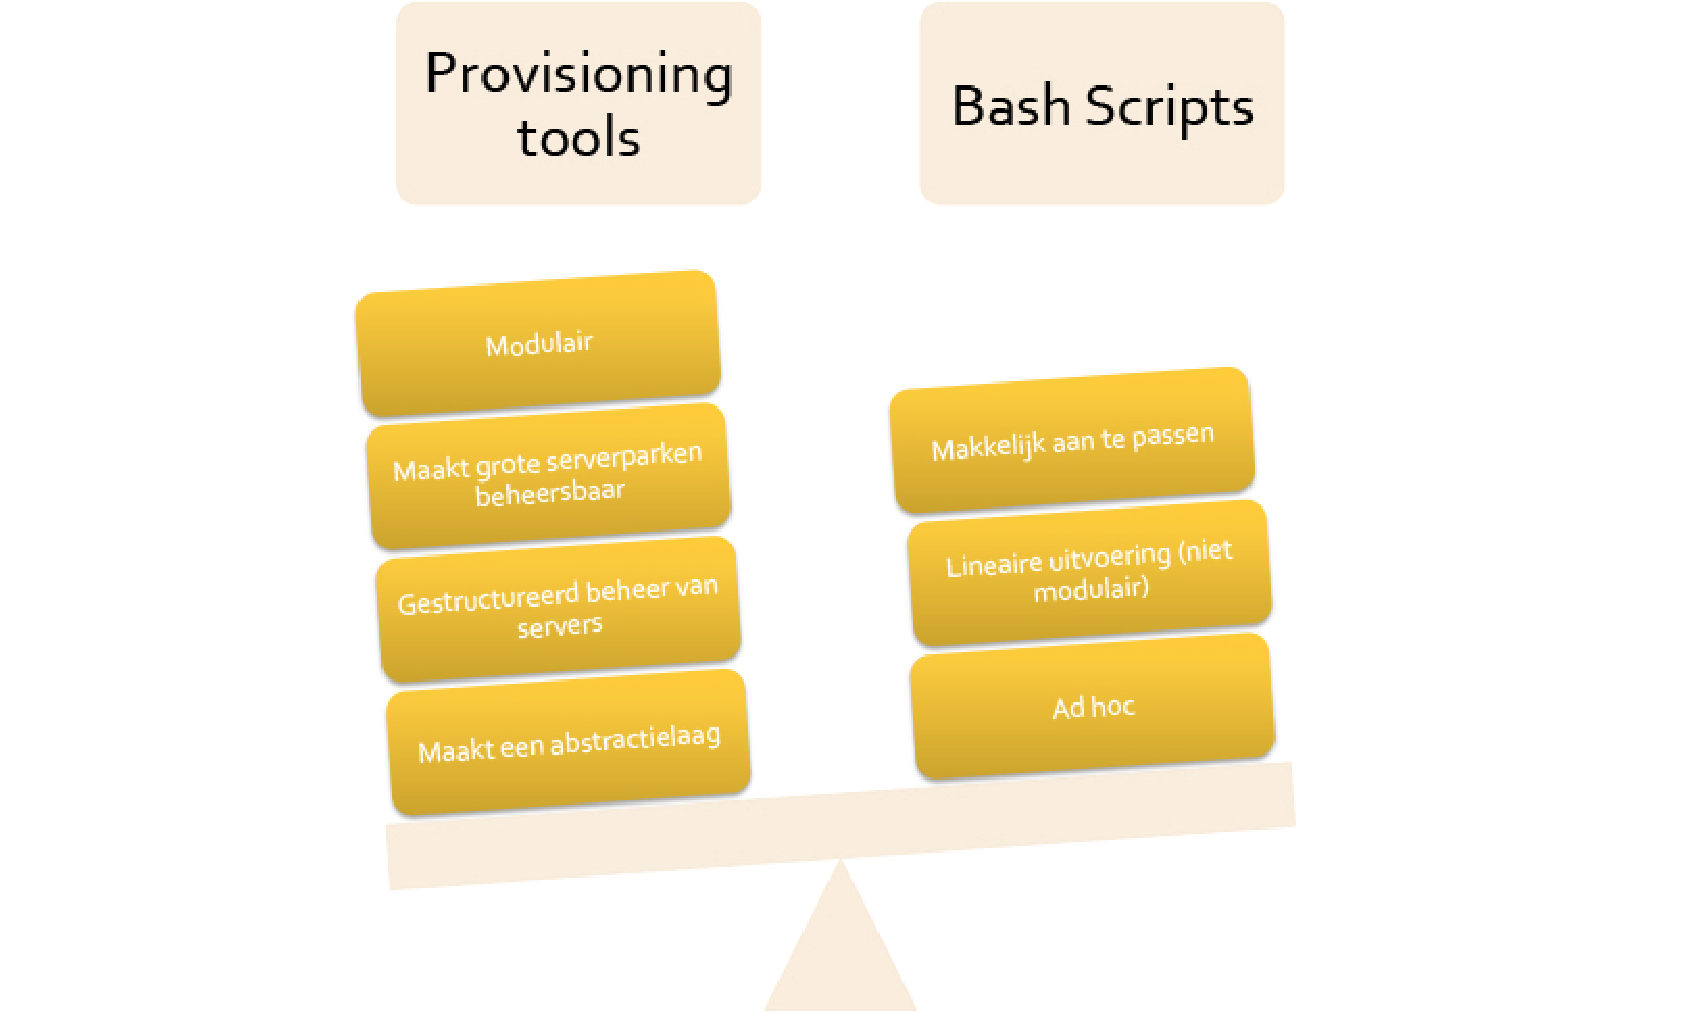
\includegraphics[scale=0.5]{overzicht.pdf}\caption{Provisioning tools versus bashscripts: een overzicht.}\label{3}
\end{figure}
\newpage
\section{Opdracht \& Werkplan}
\subsection{Opdracht}
In eerste instantie is het mijn opdracht om een analyse te maken van de bestaande populaire
`state-of-the-art' provisioning tools (Ansible, Chef, Salt \& Puppet) en te kijken welke van hen het beste passen bij
de noden en de financiële mogelijkheden van het bedrijf.\\

\noindent Vervolgens is het de bedoeling om deze ook in de praktijk
te gaan uittesten met als verhoopt resultaat enkele werkende provisioning configuraties voor Yesplan voor een paar provisioning 
tools. Alle provisioning tools hebben standaard configuraties beschikbaar voor 
zeer klassieke opstellingen (Bv. een server die Apache, PHP en MySQL draait), 
maar voor het maken van een provisioning configuratie voor Yesplan zullen er 
sowieso uitbreidingen moeten geschreven worden. Yesplan gebruikt namelijk een erg specifieke ontwikkelomgeving voor hun applicatie, met 
name Gemstone/S 64 Bit, kortweg een variant van Smalltalk. Geen enkele van de bestaande provisioning tools biedt de configuratie 
van deze ontwikkelomgeving standaard aan. Ook de Yesplanapplicatie zal als 
uitbreiding moeten integreren met deze provisioning tools.\\

\noindent Bijna alle provisioning tools hebben een website waarop gebruikers
hun geschreven uitbreidingen kunnen delen met andere gebruikers. Deze stage heeft dan ook een `open source'-component: 
vermits ik voor enkele 
provisioning tools uitbreidingen zal schrijven om de installatie van hun ontwikkelomgeving te automatiseren, te configureren en te beheren,  is het de bedoeling om deze 
uitbreidingen ook gratis aan te bieden op deze websites. Zodoende kunnen ontwikkelaars die een 
serverconfiguratie nodig hebben waarop gsDevKit (Gemstone/S 64 Bit) moet draaien, mijn uitbreidingen gebruiken
en moet na mij niemand dat wiel nog gaan heruitvinden. Dit `open source'-component komt er 
ook niet helemaal toevallig: stagementor Johan Brichau helpt zelf actief mee aan de 
ontwikkeling van Gemstone/S 64 Bit en het aanbieden van zulke uitbreidingen die 
het installatieproces op een server automatiseren, zou de populariteit van de 
ontwikkelomgeving lichtjes kunnen verhogen. Het huidige installatieproces is immers vrij ingewikkeld.\\


\end{itemize}

\subsection{Werkplan}
We kunnen volgende fases duidelijk onderscheiden:

\begin{enumerate}
  \item Analyse maken van de verschillende provisioning tools, hun voor- \& 
  nadelen afwegen voor het bedrijf.
  \item In meest passende provisioning tools uitbreidingen ontwikkelen die de 
  installatie van gsDevKit (Gemstone/S 64 Bit) automatiseren.
  \item De meeste provisioning tools hebben een website om zelfgeschreven 
  uitbreidingen op uit te wisselen. Mijn gemaakte uitbreidingen voor de 
  ontwikkelomgeving gsDevKit moeten hierop worden gepubliceerd.
  \item Eens gsDevKit samenwerkt met de uitgekozen provisioning tools, moeten 
  er nu uitbreidingen geschreven worden om ook de Yesplanapplicatie te laten 
  runnen via de provsioning tools.

  \item Eens de configuratie op deze provisioning tools werkt, zou hun werking moeten 
  gesimuleerd worden via het draaien van meerdere virtuele machine's. Met een simulatie met meerdere virtuele machine's
  kunnen we immers een opstelling van een serverpark nabootsen en kijken wel efficiëntiewinsten een provisioning tool nu echt levert bij het beheer
  van serverparken.
    
    \item De opdrachten 2-5 moeten worden uitgevoerd voor een aantal verschillende provisioning 
    tools. Zeker de provisioning tools die tijdens de analyse uit opdracht 1 als geschikt worden 
    bevonden, moeten aan bod komen.
    
    \end{enumerate}
\newpage
\section{Gebruikte technologie}
\subsection{Puppet}
\subsubsection{Algemene beschrijving}
Puppet is een configuratiemangement-systeem dat provisioning 
toelaat op Unix-achtige \& Microsoft Windows-systemen. Om de gewenste systeemconfiguratie 
te beschrijven, biedt Puppet een declaratieve scriptingtaal aan. Puppet is gratis 
voor serverparken kleiner dan 10 servers. Daarna moet er per server worden
bijbetaald. In de praktijk betekent dit Puppet gratis te gebruiken is voor testdoeleinden,
maar in een echt serverpark bijna steeds betalend is. Provisioning is  meestal pas commercieel 
interessant vanaf een serverpark groter dan 10 servers. Sommige delen van Puppet zijn vrijgegeven onder open source, maar om als
professioneel bedrijf echt je voordeel te doen met provisioning via Puppet, moet je steeds
een betalende licentie aanschaffen, de vrijgegeven delen in open source volstaan immers niet voor bedrijfstoepassingen.\\

\noindent Puppet is zonder twijfel de meest populaire provisioning tool op dit 
moment. Grote spelers zoals de Wikimedia Foundation, Reddit, Twitter, Paypal, 
Citrix, Spotify, Oracle, Google,... gebruiken allemaal Puppet om hun 
serverparken mee te beheren. In figuur \ref{workflow} vind je alvast een 
standaard workflow om met Puppet te werken.

\begin{figure}[h!]
  \centering
  \includegraphics[scale=0.6]{workflow.png}\caption{De workflow van Puppet (Figuur gedownload van \emph{http://www.puppetlabs.com/})}\label{workflow}
\end{figure}



\subsubsection{Architectuur}
\paragraph{Puppet master beheert meerder Pupppet agents}
Een typische architectuur van Puppet die een serverpark beheert omvat een \emph{Puppet master}, een soort 
van hoofdserver die alle andere servers, de \emph{Puppet agents}, bestuurt. Een 
overzicht van deze verhouding vind je in Figuur \ref{overzicht}. Om als server een Puppet agent te 
worden onder de controle van een Puppet master, moet de server gemount worden 
met een besturingsyssteem (Unix-achtig of Microsoft Windows) en moet daarop de 
Puppet agent-software geïnstalleerd worden. Indien deze server vervolgens in 
het netwerk gedetecteerd kan worden door de Puppet master, kan de 
feitelijke provisioning plaatsvinden en kan de server als agent van de master fungeren. Het mounten van servers en deze klaarmaken 
om als agent van een Puppet master te functioneren, is een proces dat - zeker in kleine tot middelgrote IT-bedrijven - meestal overgelaten 
wordt aan een hostingbedrijf. De meeste hostingbedrijven hebben trouwens ook op hun beurt 
automatische procedures om Puppet master-agents architecturen op te zetten. Eens 
een server als Puppet agent fungeert, vraagt het aan de Puppet master om de 
relevante configuratie-informatie te krijgen. Vervolgens geeft de Puppet master 
de juiste, nodespecifieke (=agentspecifieke), informatie door en krijgt het constant updates over de toestand van de 
agent. Zo ontstaat er een permanente wisselwerking.
\begin{figure}[h]
  \centering
  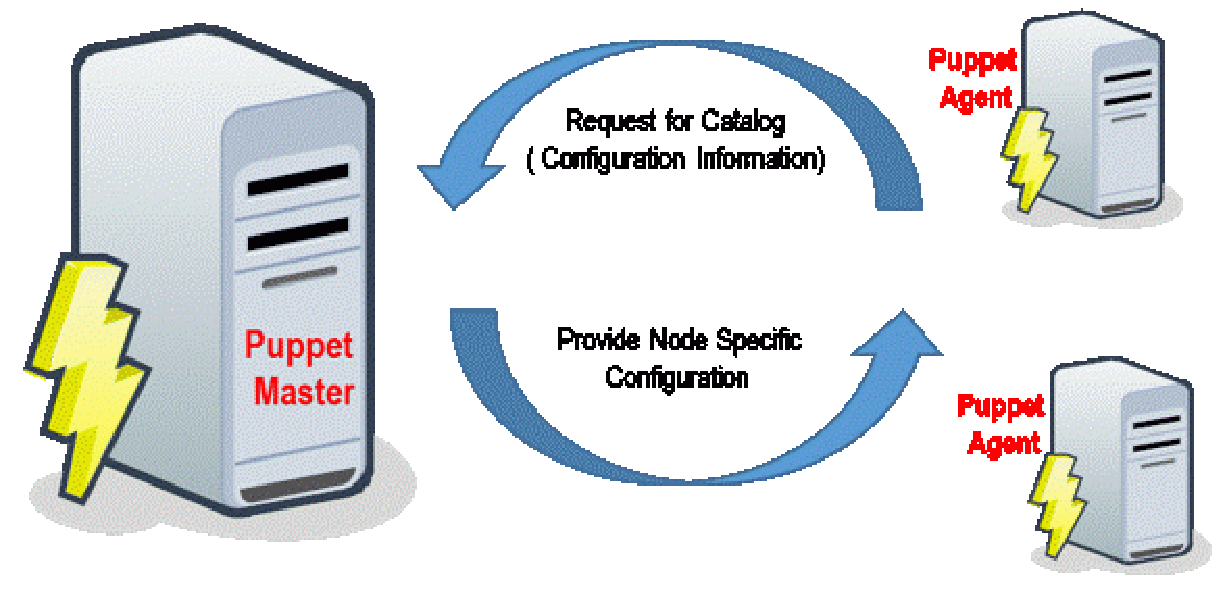
\includegraphics[scale=0.4]{puppetoverzicht.pdf}\caption{De verhouding tussen de Puppet Master en meerdere Puppet Agents. (Figuur gedownload van \emph{http://www.gocit.vn/})}\label{overzicht}
\end{figure}

\paragraph{Nodespecifieke informatie}
We gaan nu iets dieper in op de `nodespecfieke' informatie die de Puppet Master 
levert. In de declaratieve scriptingtaal \emph{Puppet code} leg je in \emph{manifests} 
vast wat de toestand van een agent moet zijn, je kan hier zogoed als alles wat 
je maar kan verzinnen in vastleggen op een declaratieve manier:

\begin{itemize}
  \item De gebruikersaccounts die op de agent moeten beschikbaar zijn en welke rechten zij hebben,
  \item De bestanden die op de agent moeten aanwezig zijn,
  \item Bepaalde instellingen die op de agent moeten ingesteld worden,
  \item Software die op de agent geïnstalleerd moet worden,
  \item enz,...
\end{itemize}

\noindent Hoewel je alles in manifests zelf kan vastleggen, ga je echter heel vaak externe 
of zelfgeschreven modules aanroepen in de manifests om de gewenste toestand van een agent te 
beschrijven. Dat maakt dat je niet alles in de manifests zelf moet regelen, maar
modules het vuile werk kunnen doen (abstractie via zwarte doos-principe). Modules zijn een op zichzelfstaand geheel van code en data om één 
bepaald doel te dienen. Zo heb je bijvoorbeeld modules om \emph{Apache} te installeren 
en te configureren op een agent, heb je modules om allerlei databanken te laten 
draaien,... Zowat elke populaire technologie die op servers moet draaien is 
intussen wel vertaald naar een kant-en-klare Puppet module. Veel van deze modules worden
publiek toegankelijk gemaakt op de PuppetForge, een soort `youtube' voor Puppet modules. Modules kunnen vaak 
ook helemaal naar de smaak van de gebruiker worden ingesteld, vermits ze 
geparametriseerd kunnen worden. \\

\noindent Elke blok code in een 
module krijgt in Puppet een naam en wordt een \emph{Puppet class} genoemd. 
Uiteindelijk wordt een module uitgevoerd door in een manifest classes van de 
module te invokeren. Puppet classes hebben voor alle duidelijkheid niets te maken met classes uit een object-georiënteerde programmeertaal.
 Uiteindelijk zijn dus Puppet manifests en Puppet modules manieren
om de configuratie requirements op agents op een gestructureerde, begrijpbare en herbruikbare manier op te slaan, maar uiteindelijk
zijn het hun codeblokken of classen die uiteindelijk voor de provisioning zorgen. Figuur \ref{o2} geeft nu een uitgebreider overzicht van de 
relatie tussen de Puppet master en meerdere Puppet agents.
\begin{figure}[h]
  \centering
  \includegraphics[scale=0.4]{o2.png}\caption{De wisselwerking tussen de Puppet master en meerdere Puppet agents. (Figuur gedownload van \emph{http://docs.puppetlabs.com/})}\label{o2}
\end{figure}

\paragraph{Puppet console} Tot slot willen we nog even de Puppet console toelichten.
Een screenshot vind je alvast in Figuur \ref{console}. Dit is een grafische webinterface dat draait op de master waarmee je een volledig overzicht krijgt van je serverpark 
met al zijn agents (nodes). Met deze web interface kan je allerlei rapporten opvragen over het slagen of falen van services,
kan je agents provisionen, agents herstellen, zoekopdrachten uitvoeren,... Zoals gezegd wordt alle configuratie-informatie 
beschreven in manifests en modules. Eens deze bouwstenen gereed zijn, is het 
mogelijk om deze via de Puppet console te combineren in eindeloze variaties door agents in diverse 
groepen onder te brengen, relaties tussen agents te leggen,... Dit maakt de 
werkelijke kracht van Puppet duidelijk: alle mogelijke serverconfiguraties zijn
weggeabstraheerd in modules en manifests, nu komt het erop aan deze gewoon te 
beheren en in te zetten waar nodig. Dit is ook voor hostinglevaranciers 
interessant, want zij kunnen bedrijven bijstaan in het beheer van hun 
serverpark, zonder zich daarom te moeten verdiepen in de gebruikte, bedrijfsspecifieke 
servertechnologieën.
\begin{figure}[h]
  \centering
  \includegraphics[scale=0.4]{puppetconsole.png}\caption{De Puppet console}\label{console}
\end{figure}
\subsubsection{Gebruik tijdens de stage}
Tijdens de stage werd er tijdens de eerste week vooral met Ansible (zie volgende paragraaf) ge\"{e}xperimenteerd, maar al snel werd het duidelijk
dat Puppet betere papieren kan voorleggen. Vooral het feit 
dat Puppet van een server verwacht dat Puppet Agent erop wordt geïnstalleerd, 
maakt veel meer abstractie mogelijk bij het provisionen. Je moet je bijvoorbeeld geen zorgen
meer maken over OS-specifieke commando's
zoals bijvoorbeeld \verb rpm , \verb apt  of \verb yum  (die allemaal hetzelfde doen maar het hangt af van het OS welke je moet gebruiken), omdat het installeren van de Puppet agent-software die verschillen
wegabstraheert. Het feit dat ook de hostingleverancier van Yesplan
zelf Puppet kent en standaard kan aanbieden, was een extra troef. De hele verdere stage
was een ontdekkingstocht met Puppet. Ik ontwikkkelde een module voor gsDevKitHome (een installatieprocedure voor Gemstone/S 64 Bit, zie verder),
een module voor de Yesplanapplicatie te installeren op een agent, een simulatie van Puppet Master met meerdere Puppet Agents via Vagrant 
en een simulatie met de Puppet Console. De module voor gsDevKitHome is 
aangeboden onder open source op de PuppetForge, het deelplatform voor Puppet 
modules en is intussen al enkele honderden keren gedownload.

\subsection{Ansible}
\subsubsection{Algemene beschrijving}
Ansible is, net zoals Puppet, een provisioning tool. Het verschil is dat Ansible 
volledig open source en dus vrij beschikbaar is. Het grote verschil met Puppet 
is hun visie dat provisioning tools \emph{minimal in nature} moeten zijn. 
Daarmee bedoelen ze dat provisioning tools geen extra dependencies op het 
serverpark mogen veroorzaken. Dat leidt ertoe dat Ansible niet verwacht dat op een 
server extra software wordt geïnstalleerd om provisioining mogelijk te maken, het beschikken over een bepaalde
Pythonversie is voldoende (dat is geen enkel obstakel, want de meeste Unixsystemen hebben dit standaard). 
Zij provisionen servers uitsluitend via SSH-commando's. Dit is een groot 
verschil met Puppet, die wel van agents verwacht dat de Puppet agent-software 
vooraf wordt geïnstalleerd. In theorie zou daarom het opzetten en provisionen van 
servers met Ansible makkelijker moeten zijn. De gewenste configuratie
wordt in Ansible beschreven in \emph{Playbooks}, de opmaaktaal waarin dat gebeurt is YAML (een soort combinatie van XML, C en Python).\\

\noindent Ansible is niet zo bekend als concurrent Puppet en is in vergelijking een erg kleine speler op de markt. 
Dat komt onder meer 
omdat ze nog maar pas vanaf 2012 bestaan, terwijl Puppet al meer dan 10 jaar op de 
markt is. De hele tool is ook nog in volle ontwikkeling en hinkt daardoor qua functionaliteit, gebruiksvriendelijkheid en ondersteuning achter op grote concurrent Puppet.
Vooral de grafische interface is bij Ansible nog niet op punt. \\

\noindent \emph{Opmerking!: Vermits Ansible slechts enkele dagen is uitgeprobeerd geweest 
gedurende de stage, laten we de beschrijving van de onderliggende architectuur 
hier weg. Het zou ons te ver leiden.}

\subsubsection{Gebruik tijdens de stage}
In de eerste week van de stage heb ik een analyse gemaakt van de verschillende 
provisioning tools en hier kwam ik tot de conclusie dat Ansible een leuke tool 
was om de stage mee te starten. Na enkele dagen uittesten, werd het echter 
duidelijk dat hun \emph{minimal in nature}-visie, dat maakt dat je geen extra
software nodig hebt om via Ansible een server te provisionen, het grote nadeel heeft dat 
je rekening moet houden met allerlei OS-specifieke verschillen en problemen. Al 
gauw werd duidelijk dat het louter via SSH-commando's provisionen toch niet zo'n 
ideale manier van werken is en dat het initieel voordeel van het niet te hoeven 
installeren van software op de servers voor het provisionen, de vele nadelen eigenlijk niet helemaal 
waard zijn. Bijgevolg werd Ansible na 2 dagen verlaten en ingeruild voor 
Puppet. Puppet verwacht zoals beschreven in de vorige paragraaf wel van agents dat ze eerst de Puppet 
agent-software installeren.

\subsection{Vagrant}
\subsubsection{Algemene beschrijving}
Vagrant is een softwarepakket voor het maken en 
configureren van virtual development environments. Het is een soort wrapper 
tussen virtualisatiesoftware (zoals VirtualBox, VMware,...) en 
configuratiemanagementsoftware (zoals de provisioning tools Puppet en Ansible). Vagrant maakt het 
dus in feite mogelijk om de provisioning tools uit te testen op servers die lokaal draaiende 
virtuele machines zijn. \\

\subsubsection{Gebruik tijdens de stage}
\noindent In de stage heb ik Vagrant altijd gebruikt. Dat is ook logisch, vermits ik uiteraard geen serverpark ter beschikking had om mee te kunnen experimenteren. Alle uitbreidingen die ik 
heb geschreven, alle provisioning tools die ik heb uitgeprobeerd, zijn 
uitgeprobeerd door servers als virtuele machines te simuleren met Vagrant en daarop de 
provisioning tools los te laten. In het begin beperkte zich dat tot één virtuele machine die geprovisioned werd. Op het einde van de stage ben ik er ook 
in geslaagd om via Vagrant een soort serverpark te simuleren waarbij één 
virtuele machine als hoofdserver (puppet master) fungeerde en de overige 
virtuele machine als agents (puppet agents). Deze simulatie was erg handig om 
het effect van provisioning te kunnen inschatten op een serverpark met meerdere 
servers.

\subsection{GsDevKit, Gemstone/S 64 Bit \& webEditionHome}
\subsubsection{Algemene beschrijving}
De Gemstone/S 64 Bit is een applicatieframework voor Smalltalk. In combinatie met 
Seaside en Topaz levert dat een ontwikkelomgeving voor dynamische 
webapplicaties. Dit is de ontwikkelomgeving die door Yesplan gebruikt om zijn planningssoftware mee te ontwikkelen.\\

\noindent GsDevkit is een pakket dat deze technologieën bundelt en installeerbaar maakt. 
webEdition was hiervan de voorganger, maar dit pakket werd tijdens de stage onbeschikbaar.
\subsubsection{Gebruik tijdens de stage}
Ik heb een module voor Puppet geschreven (zie verder) om gsDevKit via provisioning op een server te 
kunnen installeren. Aanvankelijk was dit echter een module voor webEdition, maar 
dit pakket werd onbeschikbaar gedurende de stage waardoor ik grote delen van de module opnieuw
moest ontwikkelen. Ik ben echter nooit met deze ontwikkelomgeving zelf aan de slag 
gegaan, mijn doel was immers louter om deze pakketten via provisioning te laten runnen op 
servers. De module werd op het einde van de stage beschikbaar gemaakt voor het 
grote publiek via de PuppetForge, een webplatform om modules voor Puppet uit te wisselen. De 
module werd intussen al enkele honderden keren gedownload.



\newpage
\section{Logboek}
In totaal werden er \textbf{23 werkdagen} gewerkt in het stagebedrijf, dat zijn 5 dagen meer dan de verplichte 18 stagedagen. Zoals u 
merkt in dit logboek, zijn de data heel erg verspreid over een duurtijd van 
meerdere maanden (het zwaartepunt van de stage lag wel in de zomer). Dit heeft 
meerdere factoren: enerzijds kon de stagementor in het bedrijf niet altijd 
beschikbaar zijn (vakantie, drukke periode, congressen,...). Stage lopen zonder zijn aanwezigheid was niet echt een optie, want ik had 
vaak heel erg specifieke, technische hulp nodig. Anderzijds was ikzelf ook vaak belet: de tweede zittijd begon sneller 
dan voorzien waardoor ik plots een week minder dan voorzien in augustus kon 
werken en in september ging ik op vakantie. De stage werd daarom in het 1ste semester hervat en
deeltijds gecombineerd met mijn lerarenstage aan het Koninklijk Atheneum van Etterbeek
die ik vervolmaakte in het kader van mijn lerarenopleiding. Die flexibiliteit 
was echter geen belemmering, maar juist een verrijking vermits de verschillende 
periodes toelieten om de probleemstelling vanuit een andere invalshoek te 
benaderen. In februari 2015 volgde nog een slotpresentatie voor de developers 
van het bedrijf waar ik hen een globaal overzicht van de stage en de resultaten 
presenteerde.
\begin{itemize}
  \item \textbf{Maandag 30 juni}: Kennismaking met de applicatie Yesplan, 
  concretisering van de doelen van de stage.
    \item \textbf{Dinsdag 1 juli}: Analyse verschillende provisioning tools.
        \item \textbf{Woendag 2 juli}: Analyse verschillende provisioning tools.    
     \item \textbf{Donderdag 3 juli}: Analyse verschillende provisioning tools. 
     Presentatie gegeven over de bevindingen.
    \item \textbf{Vrijdag 4 juli}: Leren werken met Ansible, de provisioning 
    tool die het beste uit de analyse kwam.
      \item \textbf{Dinsdag 8 juli}: Leren werken met Ansible.
    \item \textbf{Woendag 9 juli}: Leren werken met Ansible, overgestapt op 
    Puppet. Ansible doet aan provisioning door SSH-commando's op servers af te 
    sturen. Dit lijkt echter enkel te werken op zeer specifieke 
    serverinstallaties. We schakelen over op Puppet, de tweede `beste' uit de 
    analyse.
    \item \textbf{Donderdag 10 juli}: Leren werken met Puppet.
     \item \textbf{Vrijdag 11 juli}: Leren werken met Puppet.
 \item \textbf{Maandag 28 juli}: Ontwikkeling van webEditionHome, een 
 installatiepakket voor gsDevKit als uitbreiding voor Puppet.
\item \textbf{Dinsdag 29 juli}: Ontwikkeling van webEditionHome.
    \item \textbf{Woendag 30 juli}: Ontwikkeling van webEditionHome.    
\item \textbf{Donderdag 31 juli}: Ontwikkeling van webEditionHome.
    \item \textbf{Vrijdag 1 augustus}: Module voor webEditionHome klaar en 
    opgeleverd.
    \item \textbf{Woensdag 8 oktober}: Terugval. webEditionHome, het installatiepakket voor gsDevKit blijkt uit 
    ontwikkeling gegaan te zijn en is niet meer beschikbaar. De werkende module 
    van augustus blijkt dan ook niet meer te werken. We beginnen opnieuw nu met 
    een nieuwer installatiepakket: gsDevKitHome.
    
    
         \item \textbf{Vrijdag 10 oktober}: Ontwikkeling gsDevKitHome.
           \item \textbf{Woensdag 15 oktober}: Ontwikkeling gsDevKitHome.
        \item \textbf{Vrijdag 17 oktober}: Simulaties maken van meerdere agents 
        en één masters a.d.hv. virtuele machines.
     \item \textbf{Woensdag 22 oktober}: Simulaties maken van meerdere agents 
        en één masters a.d.hv. virtuele machines.
     \item \textbf{Vrijdag 24 oktober}: Simulatie gemaakt van de Puppet Web 
     Interface.
        \item \textbf{Woensdag 19 november}: Namiddag samengezeten rond Yesplanintegratie 
        in de gemaakte provisioningscripts.
        \item \textbf{Maandag 16 februari}: Slotpresentatie bij Yesplan.

\end{itemize}

\newpage
\section{Behaalde resultaten}
We overlopen elk punt van het werkplan.
\begin{enumerate}
\item Analyse maken van de verschillende provisioning tools, hun voor- & nadelen afwegen voor het 
bedrijf.\\

\noindent \textbf{Gelukt} \includegraphics[scale=0.15]{gelukt.pdf}. In de eerste week van de stage werd hierover een 
presentatie gegeven. Ansible en Puppet kwamen als meest geschikt uit de bus. 
\item In meest passende provisioning tools uitbreidingen ontwikkelen die de installatie van gsDevKit 
automatiseren.\\

\noindent \textbf{Gelukt} \includegraphics[scale=0.15]{gelukt.pdf}. Er werd een 
Puppet module geschreven voor gsDevKit.

\item  De meeste provisioning tools hebben een website om zelfgeschreven uitbreidingen op uit te wisselen. 
Mijn gemaakte uitbreidingen voor de ontwikkelomgeving gsDevKit moeten hierop worden 
gepubliceerd.\\

\noindent \textbf{Gelukt} \includegraphics[scale=0.15]{gelukt.pdf}. De gsDevKit 
module voor Puppet werd op PuppetForge (een website om Puppet modules uit te wisselen) vrij beschikbaar gemaakt.

\item Eens gsDevKit samenwerkt met de uitgekozen provisioning tools, moeten er nu uitbreidingen geschreven worden om ook 
de Yesplanapplicatie te laten runnen via de provsioning tools.\\

\noindent \textbf{Gelukt} \includegraphics[scale=0.15]{gelukt.pdf}. Er werd een 
Puppet module geschreven voor de Yesplanapplicatie. Deze steunt onderliggend op de 
gsDevKit module en nog enkele third party modules van de Puppet forge (onder andere een module om repositories van Github te halen, module
voor de websserver Nginx,...).

\item  Eens de configuratie op deze provisioning tools werkt, zou hun werking moeten gesimuleerd worden via virtuele machine’s 
zodanig dat de mogelijkheden om meerdere servers te beheren kan getest worden.\\

\noindent \textbf{Gelukt} \includegraphics[scale=0.15]{gelukt.pdf}. Via Vagrant 
werd er een simulatie gemaakt van een Puppet master die meerdere Puppet agents 
beheert. Zowel de master als de agents zijn in deze simulatie virtuele machines die worden gerund 
met Vagrant. Hiermee hebben we dus eigenlijk een serverpark gesimuleerd.

    \item De opdrachten 2-5 moeten worden uitgevoerd in een aantal verschillende provisioing 
    tools. Zeker de provisioning tools die tijdens de analyse uit opdracht 1 als geschikt worden 
    bevonden, moeten aan bod komen.\\
    
    \noindent \textbf{Gefaald} \includegraphics[scale=0.15]{gefaald.jpg}. Hoewel er wel kort
    met Ansible is geëxperimenteerd, bestaat het opgeleverde werk enkel uit 
    modules, manifests en simulaties met Puppet. Het schrijven van de module 
    voor gsDevKit nam uiteindelijk veel meer tijd in beslag dan verhoopt, 
    doordat die installatieprocedure in het begin heelwat problemen gaf als Puppet module.  Daardoor moest ik vaak
    samen met de stagementor op zoek naar oplossingen voor vaak erg vieze en specifieke errors. Ook het feit dat het webEditionHome-project
    bij mijn terugkeer in oktober intussen was stopgezet en ik mijn module dus moest herschrijven naar gsDevKit heeft veel vertraging opgeleverd. Er was uiteindelijk geen
    tijd meer om nog andere provisioning tools uit te spitten of de 
    werkzaamheden in Ansible te hervatten.
       \end{enumerate}
    
\section{Zelfevaluatie}
Als positieve punten denk ik dat ik mag stellen dat ik:
\begin{itemize}
  \item ... altijd duidelijke afspraken heb gemaakt over wanneer ik wel en niet kon 
  komen werken,
  \item ... de belangrijkste doelstellingen van de stage gerealiseerd heb.,
  \item ... vrij betrouwbaar ben (op één overmacht na, waarbij ik de eindpresentatie nog de dag voordien heb
  moeten verplaatsen wegens problemen met leden van een groepswerk) op het 
  naleven van deadlines en afspraken.
  \item ... ondanks de erg drukke tijden (in de zomer had ik tweede zit, in oktober combineerde ik de stage
  met de stage uit de lerarenopleiding), deze stage hier nauwelijks tot eigenlijk helemaal niet onder geleden heeft. 
\end{itemize}
Toch is er, zoals steeds, zeker nog ruimte voor verbetering, moest ik de stage 
opnieuw doen dan zou ik:
\begin{itemize}
  \item ... mij iets meer verdiepen in sommige vaardigheden die toch wel nuttig waren geweest. 
  \begin{itemize}
   \item Zo moest ik bijvoorbeeld enorm veel met de Terminal werken, terwijl ik eigenlijk maar enkele maanden voor
  de stage een Mac gebruiker ben geworden (daarvoor Windows). Ik heb heelwat tijd verloren door gewoon niet goed 
  genoeg de verschillende commando's te kennen. Had ik gewoon eens een 
  namiddagje tijdens de stage uitgetrokken om mijzelf de belangrijkste 
  commando's aan te leren, dan had dat vermoedelijk heelwat tijd kunnen besparen nadien.
  \item Ik had me ook iets beter moeten verdiepen in de feitelijke werking van 
 gsDevKit (Gemstone/S 64 Bit) vooral met betrekking tot zijn installatieproces.  Eigenlijk zou
  ik dat installatieproces eerst moeten geprobeerd hebben op mijn computer, zonder provisioning of andere extra's, om
  dan pas de module voor Puppet te schrijven. Dit had 
  heelwat vragen om hulp bij mijn stagementor kunnen vermijden. Ik was iets 
  teveel gefocust op de mogelijkheden van Puppet en ben dan ook direct aan het schrijven van de module begonnen, terwijl een betere kennis van 
  gsDevKit globaal gezien tijd had kunnen besparen.
 
  \end{itemize}
  
    \item ... proberen soms wat meer door te werken. Het feit dat de stage 
    meteen begon na een immens drukke periode en ook gecombineerd werd met de tweede zit en later met de lerarenstage, maakte het soms verleidelijk om 
    een beetje lui te zijn. Ik was me hier wel heel goed van bewust en heb dat tot een minimum proberen te beperken.
    Om die reden ben ik ook nauwelijks (slechts 1 dag) ingegaan op het aanbod van de stagementor om sommige dagen
    van thuis uit te werken, maar ben ik zogoed als altijd op de stageplaats geweest. 
    Van thuis uit werken zou immers mijn productiviteit serieus gefnuikt 
    hebben.
\end{itemize}
\newpage
\section{Reflectie \& Slotbeschouwing}
Als ik terugblik op de stage, dan was het een erg leerrijke periode waarbij ik 
het in eerste instantie aangenaam vond om de werking van een start-up van nader bij te mogen meemaken. 
\\

\noindent Ik heb altijd al zin gehad om zelf ooit een informaticabedrijfje op te 
starten. In de media verschijnen vaak verhalen van erg succesvolle start-ups 
zoals Snapchat, Tinder,... die met een heel simpel idee de hele wereld veroveren en hun bedrijf na enkele jaren
met een miljoenenwinst kunnen doorverkopen. Toch is dat sprookje voor slechts de happy few weggelegd en lijkt het voor mezelf
veel realistischer om er een bepaalde sector uit te pikken (bv. de vastgoedsector, gehandicaptenzorg,...) en daarvoor
gespecialiseerde software te ontwikkelen. Je hoeft dan ook niet eeuwen te wachten op het `perfecte idee' om een bedrijf rond op te richten,
er zijn sectoren genoeg die softwarematig nog in de middeleeuwen vertoeven. Idealiter start je bedrijf dan als een soort spin-off van een bedrijf in die sector. Yesplan
 is hierin voor mij een absoluut een voorbeeld: begonnen in de schoot van de Vooruit, bouwt het intussen succesvolle planningssoftware voor allerhande
 cultuurhuizen. Zo zie je dat de focus leggen op een specifieke sector vaak een succesvol business model kan opleveren.\\

\noindent Wat me daarnaast ook opviel was hoe een informele werksfeer met slechts een aantal 
programmeurs een heel efficiënt ontwikkelingsproces oplevert. Elke developer kan bij Yesplan werken op zijn eigen manier en
je kan ook van van thuis uit werken indien je dat wenst.  Wanneer een 
developer in de problemen zit, wordt er spontaan samengezeten met een andere 
developer om het probleem samen te bekijken. Ook vergaderingen worden vaak (niet allemaal) 
spontaan samengeroepen en dit enkel indien dat noodzakelijk is. Ik geloof dat 
enkel de wekelijkse devlopmeeting de enige `vaste' vergadering is. Het ontbreken van een logge, inefficiënte vergadercultuur (dat bij veel andere bedrijven
wél aanwezig is) vond ik 
een zeer positief punt in dit bedrijf. Daarnaast valt het ook op dat in een start-up het medebeslissingsrecht van een developer erg groot is:
doordat de groep developers zeer klein is, kan iedereen zijn mening geven en een werkelijke invloed hebben op het eindproduct. Dit is in grote bedrijven vaak niet zo,
daar zijn de developers vaak louter uitvoerders van design beslissingen van hogerhand. \\

\noindent Daarbuiten heb ik ook erg veel opgestoken over serverconfiguratie en het beheer 
van serverparken aan de hand van provisioning tools. Ik zou nu zonder problemen een 
serverpark kunnen opzetten en beheren met Puppet. Ook uitbreidingen schrijven 
voor Puppet is geen enkel probleem. Doordat ik tijdens de stage servers en 
serverparken steeds heb moeten simuleren, is mijn kennis over virtualisatie en 
zeker van bepaalde tools zoals Vagrant aanzienlijk toegenomen. Het valt me ook op dat de leercurve voor een nieuwe
technologie bij mij steeds gemiddeld zo'n 2 weken duurt, dat zijn dan 2 weken waarin er maar heel traag resultaten worden geboekt. Eén keer
ik het echter doorheb, kan ik veel, veel sneller werken. Dat was zeker met Puppet het geval: in het begin ging dat heel traag, maar 
nu zou ik echt heel snel nieuwe modules kunnen schrijven.\\

\noindent Conclusie: Ook al werd de stage doorlopen in erg drukke tijden, het was een 
mooie ervaring waarbij ik naast technische kennis, ook bedrijfseconomisch de 
werking van start-up heb kunnen leren kennen, het zou alvast een mooie inspiratie voor later kunnen zijn.

\noindent 




 \end{document}

